\documentclass[dvipdfmx]{article}

\usepackage[a4paper, margin=2cm]{geometry}
\usepackage[dvipdfmx]{graphicx}

\title{Intensifying Magnets with Optimization of Magnetic Dipole directions}
\author{Hirano Takeshi \thanks{hyranno4pub@gmail.com http://uncotechhack.net}}
\date{2020/03/26}

\begin{document}

\maketitle

\begin{abstract}
Arranging some magnets can intensify its magnetic field, as known as Halbach array.
Magnets can be considered as a 3 dimensional array of magnetic dipoles.
Optimizing these magnetic dipole directions, magnets can be more stronger.
This article shows how to ditermine these directions, and how to magnetize ferromagnetic material with that directions.
\end{abstract}

\section{Background}
Magnets are used for conversion between force and electricity, like motor and generator.
These devices can be more efficient, powerful, smaller, lighter, or cheaper with optimizing magnets.
Arranging magnets into Halbach array is one of the methods to achieve that.
On the other hand, magnet itself can be considered as a 3 dimensional array of magnetic dipoles.
So scaling down magnets to magnetic dipoles, it can be said that optimizing these magnetic dipole directions can intensify the magnet.



\section{Basic Situation}
In this section, we consider a basic situation that maximize the magnetic field at point $P_{f}$, toward vector $\overrightarrow{v_{f}}$.

\subsection{Determining direction}
\subsubsection{Method}
Magnetic flux density $\overrightarrow{dB}$ at point $P$ from magnetic dipole moment $\overrightarrow{dM}$ at point $P_{m}$ can be represented as below.

\begin{eqnarray}
	\overrightarrow{dB(P)} = k \nabla \frac{ \overrightarrow{dM(P_{m})} \cdot \overrightarrow{(P-P_{m})} }{ \left|\overrightarrow{(P-P_{m})}\right|^3 }
	\label{eq:dB}
\end{eqnarray}

Here, $k$ is a constant number.

Therefore, to maximize the magnetic field at point $P_{f}$, toward vector $\overrightarrow{v_{f}}$,
	solving equation below for $\overrightarrow{dM}$ gives the direction that the magnetic dipole at $P_{m}$ should take.

\begin{eqnarray}
	\overrightarrow{v_{f}} \cdot \overrightarrow{dB(P_{f})} = \left| \overrightarrow{v_{f}} \right| \left| \overrightarrow{dB(P_{f})} \right|
	\label{eq:directioneq}
\end{eqnarray}


\subsubsection{Results}
For example here, we consider a cylinder shaped magnet which fills $-5<z<5$ and $\sqrt{x^2 + y^2} < 10$.
For $P_{f}=(0,0,10)$ and $\overrightarrow{v_{f}}=(0,0,-1)$, magnetic flux density with or without optimization of magnetic dipole directions have been calculated.
Results are calculated with Maxima, then drawn with Gnuplot.

Direction of the magnetic dipoles is shown as equation\ref{eq:dMdir}.
Intensity of the magnetic dipoles are constant number depending on saturation magnetic moment of the material.

\begin{eqnarray}
	\left( 3P_{mx}(P_{mz}-10), 3P_{my}(P_{mz}-10), (P_{mz}-10)^2 - 2P_{mx}^2 - 2P_{my}^2 \right)
	\label{eq:dMdir}
\end{eqnarray}

Figure\ref{fig:simulation_opt} shows the magnetic flux density with optimization of magnetic dipole directions.
Figure\ref{fig:simulation_straight} shows the magnetic flux density with uniformed magnetic dipole directions, for comparison.

\begin{figure}[htbp]
  \begin{center}
    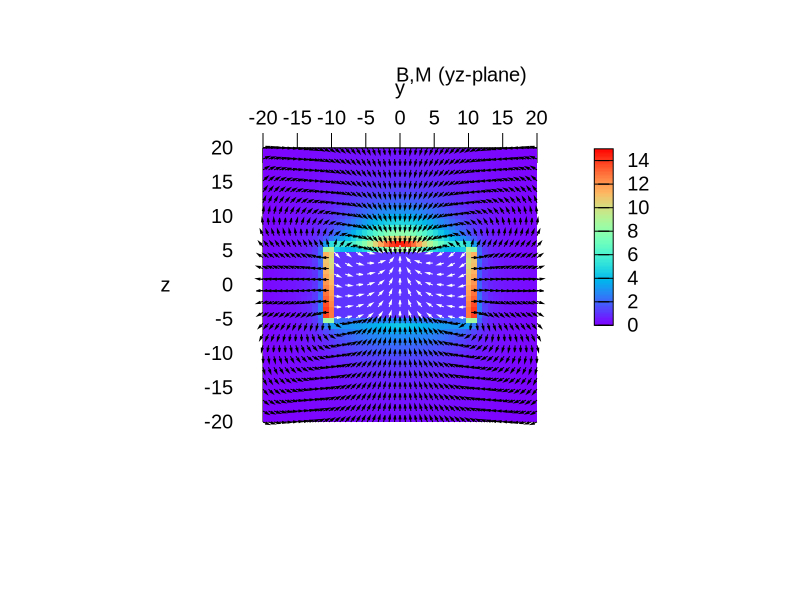
\includegraphics[clip, width=0.9\hsize, bb=100 200 600 600]{./resources/BM.svg}
    \caption{Magnetic flux density with optimization of magnetic dipole directions}
    \label{fig:simulation_opt}
  \end{center}
\end{figure}

\begin{figure}[htbp]
  \begin{center}
    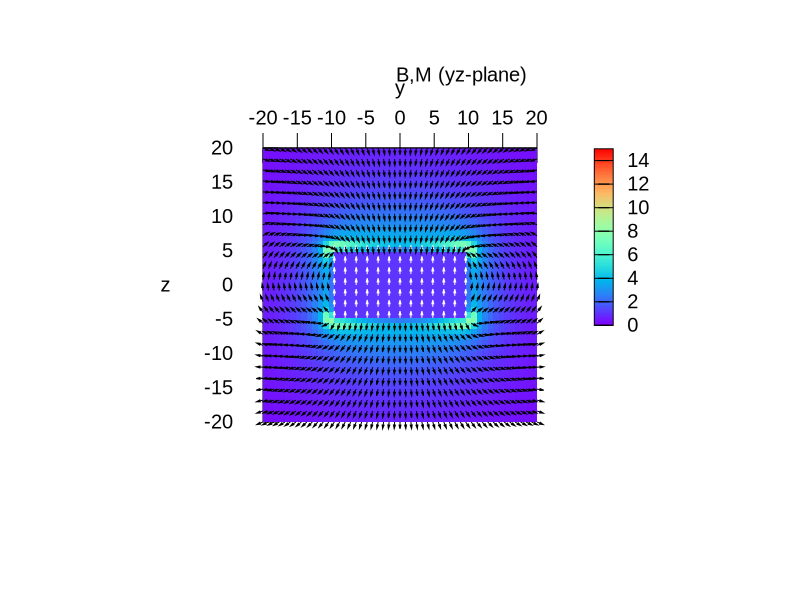
\includegraphics[clip, width=0.9\hsize, bb=100 200 600 600]{./resources/BM_straight.svg}
    \caption{Magnetic flux dinsity with uniformed magnetic dipole directions}
    \label{fig:simulation_straight}
  \end{center}
\end{figure}

In figure\ref{fig:simulation_opt} and figure\ref{fig:simulation_straight},
white arrows show directions of magnetic dipoles,
black arrows show directions of magnetic flux density,
and color show intensity of magnetic flux density.
Magnetic flux density inside magnet are not calculated.

Difference between figure\ref{fig:simulation_opt} and figure\ref{fig:simulation_straight} at the point $(0,0,10)$
is not so dramatic as near the point $(0,0,5)$,
but intensity of magnetic flux density at the point $(0,0,10)$ in figure\ref{fig:simulation_opt} ($>3.2$)
is still larger than in figure\ref{fig:simulation_straight} ($<2.6$).



\subsection{Magnetization}
I show two methods here to magnetize the magnet in these direction,
the voxel method and the single magnetic dipole method.

The voxel method means simply to magnetize indivisual magnet voxels and then combine them.
If you construct the magnet with a 3D printer,
this method can be applied with attaching magnetizing coil to the nozzle of the printer.

The single magnetic dipole method uses a magnetizing coil as a magnetic dipole.
To magnetize in proper direction, magnetic flux density $B_{c}$ from the coil should fit the equation\ref{eq:magnetizeBc}.

\begin{eqnarray}
	\overrightarrow{dM(P_{m})} \cdot \overrightarrow{B_{c}(P_{m})} = - \left| \overrightarrow{dM(P_{m})} \right| \left| \overrightarrow{B_{c}(P_{m})} \right|
	\label{eq:magnetizeBc}
\end{eqnarray}

Putting the coil as a magnetic diole at the point $P_{f}$ to the direction $-v_{f}$,
the direction of the magnetic flux density from this coil is shown as equation\ref{eq:Bcdir}.

\begin{eqnarray}
	-\left( 3P_{mx}(P_{mz}-10), 3P_{my}(P_{mz}-10), 2(P_{mz}-10)^2 - P_{mx}^2 - P_{my}^2 \right)
	\label{eq:Bcdir}
\end{eqnarray}

Comparing with equation\ref{eq:dMdir}, this is not perfect, but can be used as a approximation.


\section{Relation with Halbach Array}

You can see the direction of the magnetic dipoles goes ``$\downarrow\rightarrow\uparrow\leftarrow\downarrow$''
 near the $P_{mz}=5$ on Figure\ref{fig:simulation_opt}.
This is a part of the Halbach Array.
Trimming this part to ``$\rightarrow\uparrow\leftarrow$'', connecting with opposing ``$\leftarrow\downarrow\rightarrow$'',
 then repeatedly copying and pasting, make the Halbach Array
 ``$\rightarrow\uparrow\leftarrow\downarrow\rightarrow\uparrow\leftarrow\cdots$''.

The period of this Halbach Array $L$ is twice length of the ``$\rightarrow\uparrow\leftarrow$'' part.
The $P_{my}$ of these ``$\rightarrow'' and ``\leftarrow$'' can be get with solving equations\ref{eq:HalbachLength}.

\begin{eqnarray}
  \left\{
    \begin{array}{l}
      P_{mx} = 0 \\
      v_{f} \cdot dM(P_{m}) = 0
    \end{array}
  \right.
  \label{eq:HalbachLength}
\end{eqnarray}

The equations\ref{eq:HalbachLength} give $P_{my}=\pm\frac{P_{mz}-10}{\sqrt{2}}$, so $L=\sqrt{2}(P_{mz}-10)$.
This implies that the optimum period of the Halbach Array can be decided with the distance from the point
 where we want to maximize the magnetic flux density.
 
 
\section{Conclusion}
Magnets can be intensified with optimization of its magnetic dipole 3D array.
Example and magnetization methods for simple situation had be shown.
Applying this to the Halbach Array, its period can be decided with the distance from the point
 where we want to maximize the magnetic flux density.


\end{document}